\section{Results and Testing}
\label{sec:results-and-testing}
This chapter will focus on the results of the project, and the testing that was carried out to evaluate the performance of the different subsystems of the project. The chapter will be divided into three sections: Mechanical Design, Electronics and Software, and Computer Vision.

\subsection{Mechanical Design}
\label{sec:mechanical-design-evaluation}

\subsection{Electronics and Software}
\label{sec:electronics-and-software-evaluation}
\todo{lcd ui profiling}
\todo{add power consumption measurements from usb for complete power - implementation maybe?}

\subsection{Computer Vision}
\label{sec:computer-vision-evaluation}
This section will examine the Computer Vision system, as discussed in \autoref{sec:computer-vision-system} and implemented in \autoref{sec:computer-vision}.

\subsubsection{Component Detection Model}
The Component Detection model was trained on a dataset of 1076 images, split into a 70-20-10 split for training, validation, and testing respectively. The dataset was augmented using the augmentations discussed in \autoref{sec:image-processing}. The model was trained using the training parameters shown in \autoref{tab:training-parameters}.

\begin{figure}[H]
    \centering
    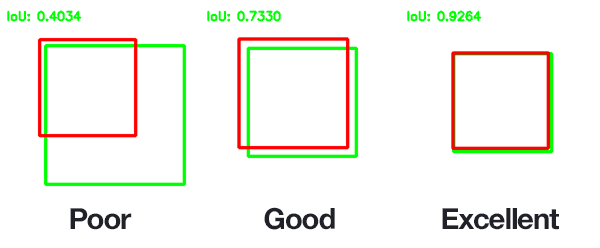
\includegraphics[width=0.8\textwidth]{imgs/articles/iou.png}
    \caption{IoU Example \cite{rosebrock_2016}}
    \label{fig:iou}
  \end{figure}
  
As discussed in \autoref{sec:real-time-object-detection}, mAP\raisebox{-1pt}{\textsuperscript{50}} is a standard metric used to evaluate object detection models. mAP\raisebox{-1pt}{\textsuperscript{50-95}} is a more rigorous metric that aggregates the mean average precision across all classes at different Intersection over Union (IoU) thresholds; in mAP\raisebox{-1pt}{\textsuperscript{50}}, an object is considered as detected if the IoU is greater than 0.5 (the predicted bounding box overlaps the ground truth bounding box by at least 50\%), whereas in mAP\raisebox{-1pt}{\textsuperscript{50-95}}, the mAP score is aggregated across different IoU thresholds from 0.5 to 0.95 in steps of 0.05. This can be seen more clearly \autoref{fig:iou}, where the second bounding box would be detected in mAP\raisebox{-1pt}{\textsuperscript{50}}, but not in mAP\raisebox{-1pt}{\textsuperscript{75}}.
  
\begin{figure}[H]
  \centering
  \includesvg[width=0.8\textwidth]{imgs/graphs/metrics_mAP50-95(B).svg} 
  \caption{TensorBoard graphing: all runs mAP\raisebox{-1pt}{\textsuperscript{50-95}} against epochs}
  \label{fig:metrics}
\end{figure}
  
In \autoref{fig:metrics}, the mAP\raisebox{-1pt}{\textsuperscript{50-95}} is shown for all training runs of the model with slightly different training parameters. It can be seen that the models tend to converge around 20 epochs, and there is a ceiling at around 80\% mAP\raisebox{-1pt}{\textsuperscript{50-95}}. This is likely due to the small dataset size, and it is made even smaller due to the use of a test set. For deployment, the training set will absorb the test set to increase the size of the dataset and improve the model's performance, however for discussion it is necessary to keep a test set separate to objectively measure the model's performance.


\begin{figure}[H]
  \centering
  \begin{minipage}[t]{0.8\textwidth}
    \centering
    \includesvg[width=\textwidth]{imgs/graphs/finalmodelmap95.svg}
  \end{minipage}
  \par\medskip
  \begin{minipage}[t]{0.8\textwidth}
    \centering
    \includesvg[width=\textwidth]{imgs/graphs/metrics_mAP50(B).svg}
  \end{minipage}
  \caption{Final Model (blue) and non-pretrained model (orange) mAP\raisebox{-1pt}{\textsuperscript{50-95}} and mAP\raisebox{-1pt}{\textsuperscript{50}} scores}
  \label{fig:final-model-metrics}
\end{figure}

As shown in \autoref{fig:final-model-metrics}, the final YOLO-OBB model (blue) achieved an mAP\raisebox{-1pt}{\textsuperscript{50-95}} of 82.8\% and an incredibly high mAP\raisebox{-1pt}{\textsuperscript{50}} of 99.5\%. This is an extremely impressive score given the relatively small size of the dataset (and made even smaller due to the need of the test set), which is truly a testament to YOLOv8's capabilities.

An experiment was run to see how the model would perform if the model was \textbf{not} pretrained on DOTOv1 \cite{9560031} given the low training time to see how much of an impact the pretraining had on the model's performance. The model, shown in orange, clearly takes much longer to converge; where the original model reaches 99.5\% mAP\raisebox{-1pt}{\textsuperscript{50}} for the first time in 18 epochs, the non-pretrained model had an mAP\raisebox{-1pt}{\textsuperscript{50}} of 82.5\%, and takes 40 epochs to reach 98\%. By the time the pretrained model achieves an mAP\raisebox{-1pt}{\textsuperscript{50-95}} of at least 80\% on epoch 26, the non-pretrained model has an mAP\raisebox{-1pt}{\textsuperscript{50-95}} of 67.4\%. This is a substantial difference, and it is clear that pretraining on a large dataset is crucial to the model's performance and training time. When the model is pretrained on a large dataset, the model is able to learn generalisable, basic features such as edge and corner detection, which are common in most images. When the model is now trained on a new dataset, it does not need to relearn these basic features, and can instead focus on learning the more complex features of the new dataset. This is known as transfer learning, and it is a common technique used in deep learning to improve the performance of models on new datasets.

\begin{figure}[H]
  \centering
  \includesvg[width=0.8\textwidth]{imgs/graphs/all.svg}
  \caption{All training runs mAP\raisebox{-1pt}{\textsuperscript{50-95}} against epochs}
  \label{fig:allruns}
\end{figure}

For completeness, the mAP\raisebox{-1pt}{\textsuperscript{50-95}} for all training runs is shown in \autoref{fig:allruns}, where the orange non-pretrained model is clearly lagging behind all other training runs.

To properly evaluate a model's performance, it is important to consider the model's performance on a test set. As described above, 10\% of the dataset was split for this, giving 98 + 10 background images for the test set.

\begin{figure}[H]
  \centering
  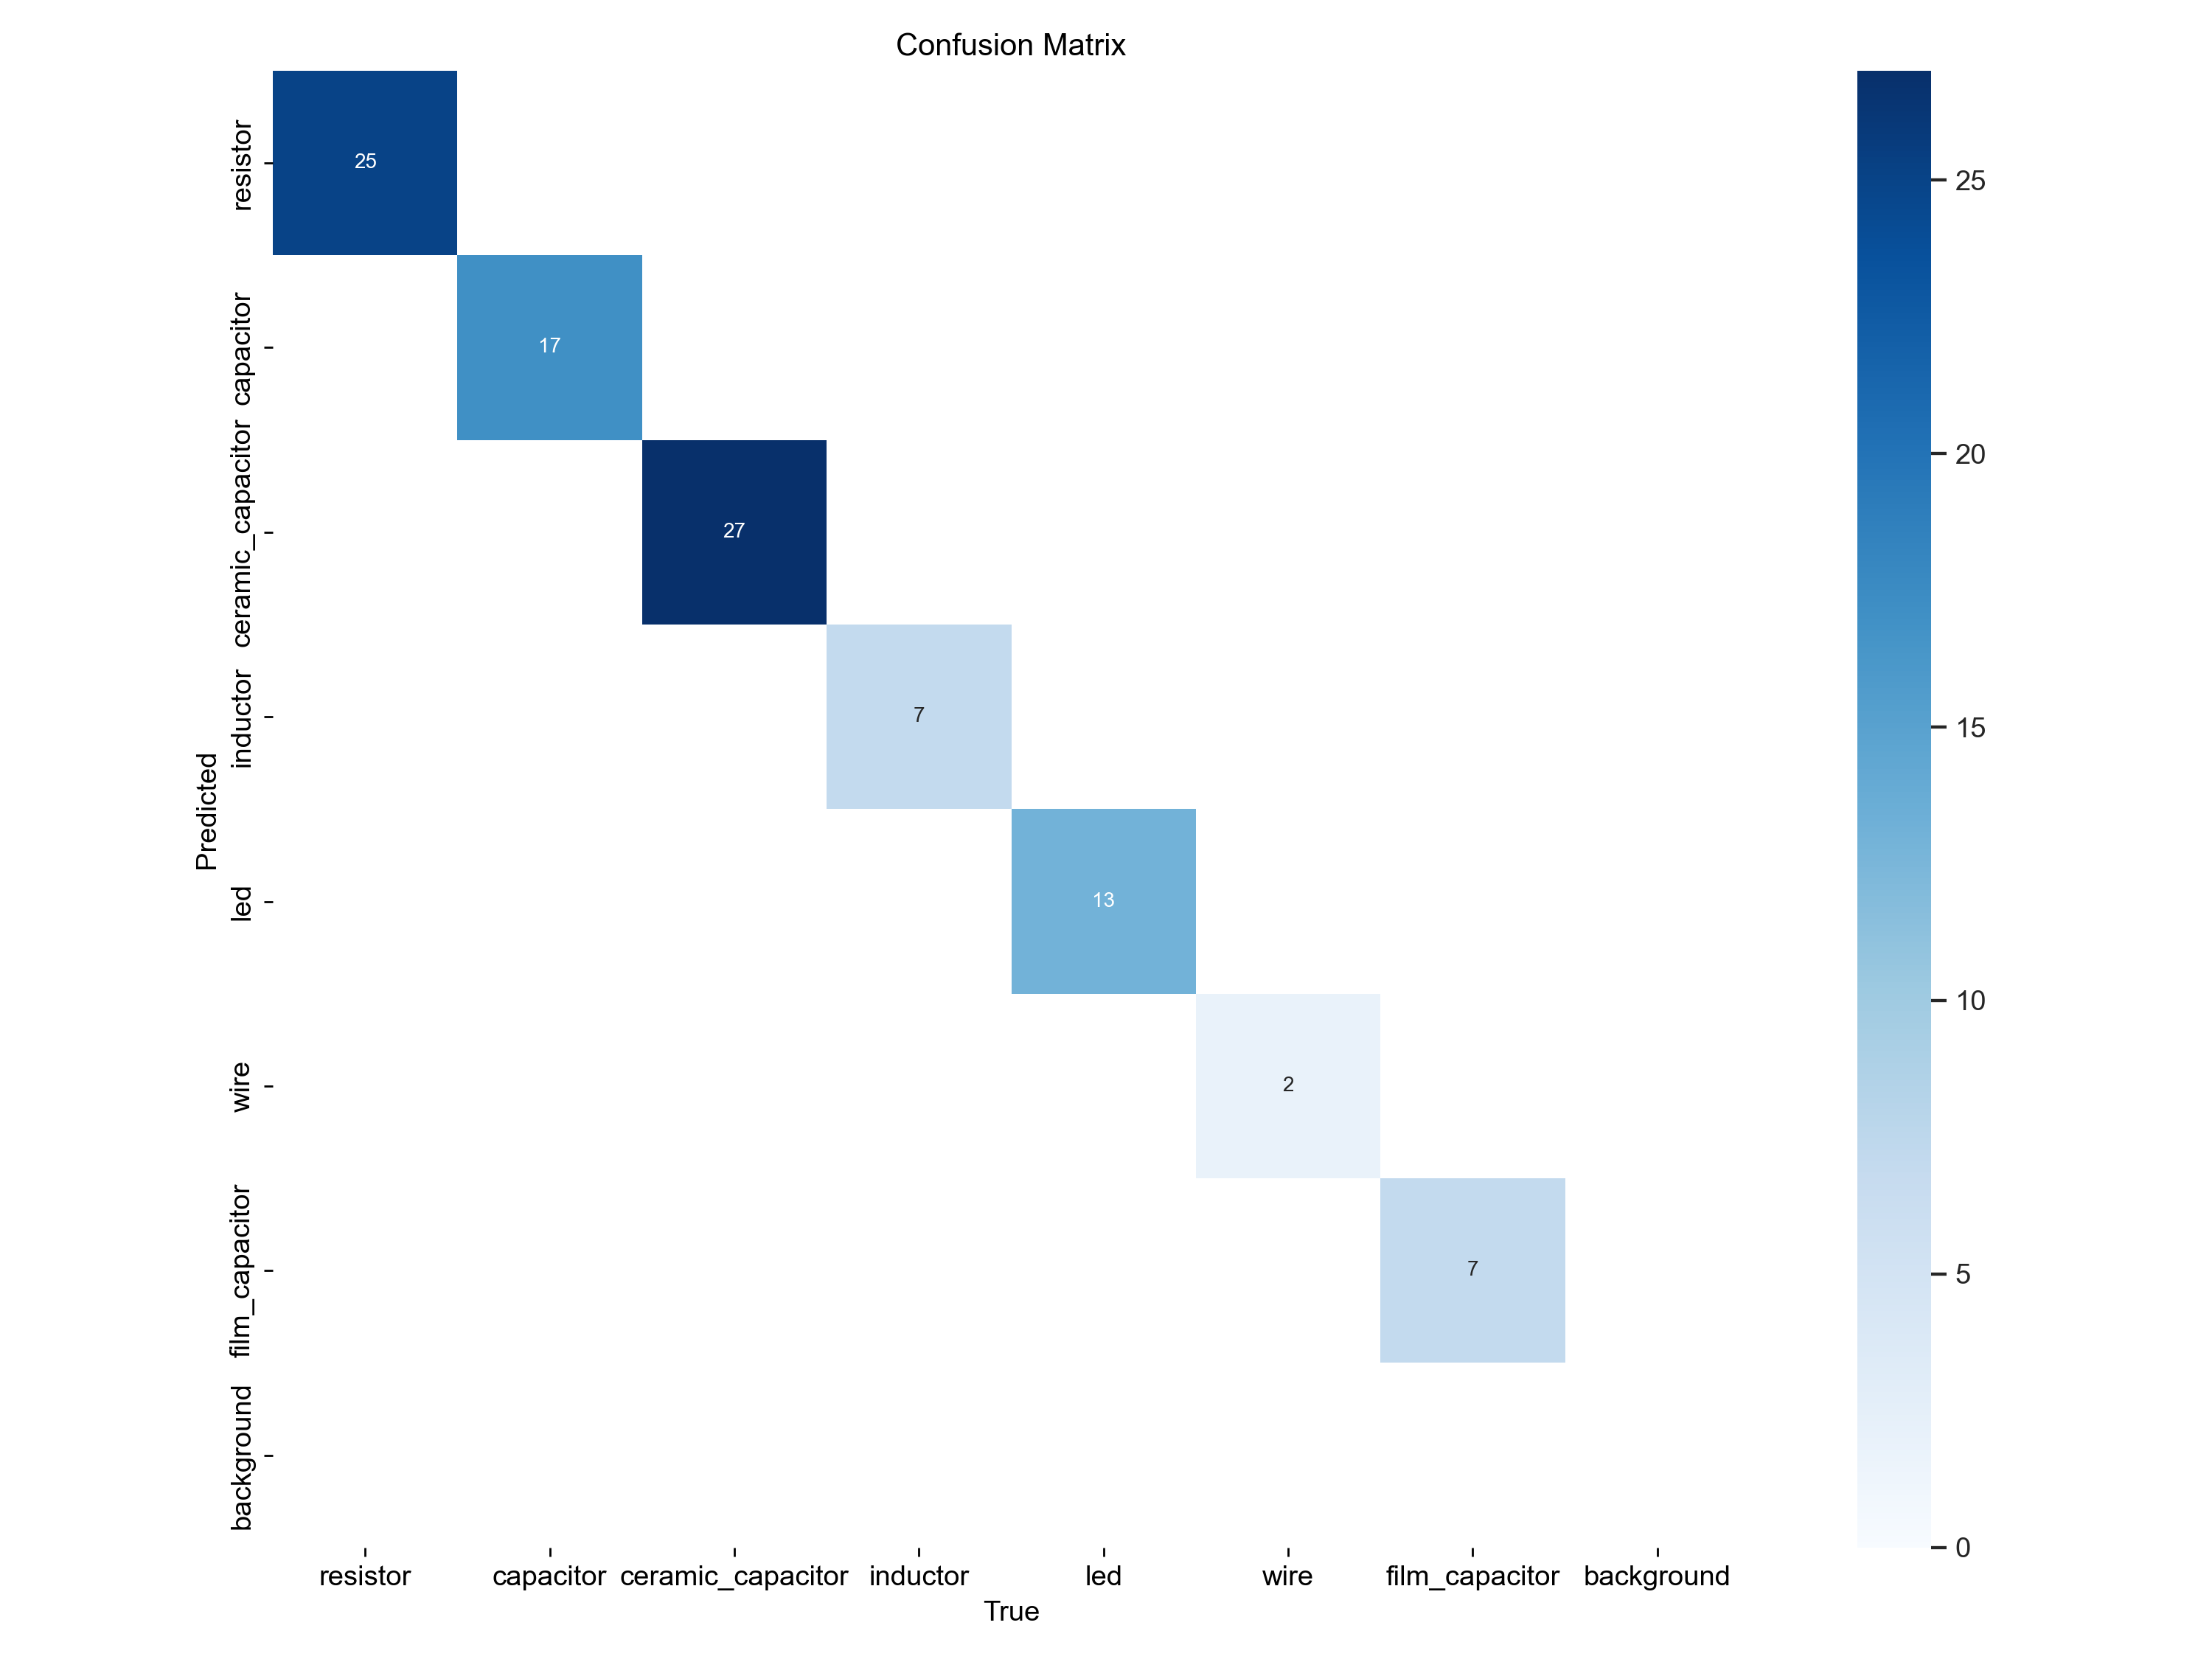
\includegraphics[width=0.8\textwidth]{imgs/graphs/confusion_matrix_final.png}
  \caption{Unnormalised confusion matrix for the test set}
  \label{fig:true-confusion-matrix}
\end{figure}

In \autoref{fig:true-confusion-matrix}, the unnormalised confusion matrix is shown, with only diagonal entries, which shows 100\% accuracy on the test set. This is a very good sign, however it is important to remember that the dataset is very small, so the validation and test set has then been used to evaluate the model, as shown in \autoref{fig:final-model-confusion-matrix}. Although the model does not learn on the validation set, it still has seen the validation set during training which may cause the model to learn features that are specific to the validation set, which is why the test set is used to evaluate the model's performance. However, showing the confusion matrix for the validation and test set will be useful in this context to show the model's performance.

\begin{figure}[H]
  \centering
  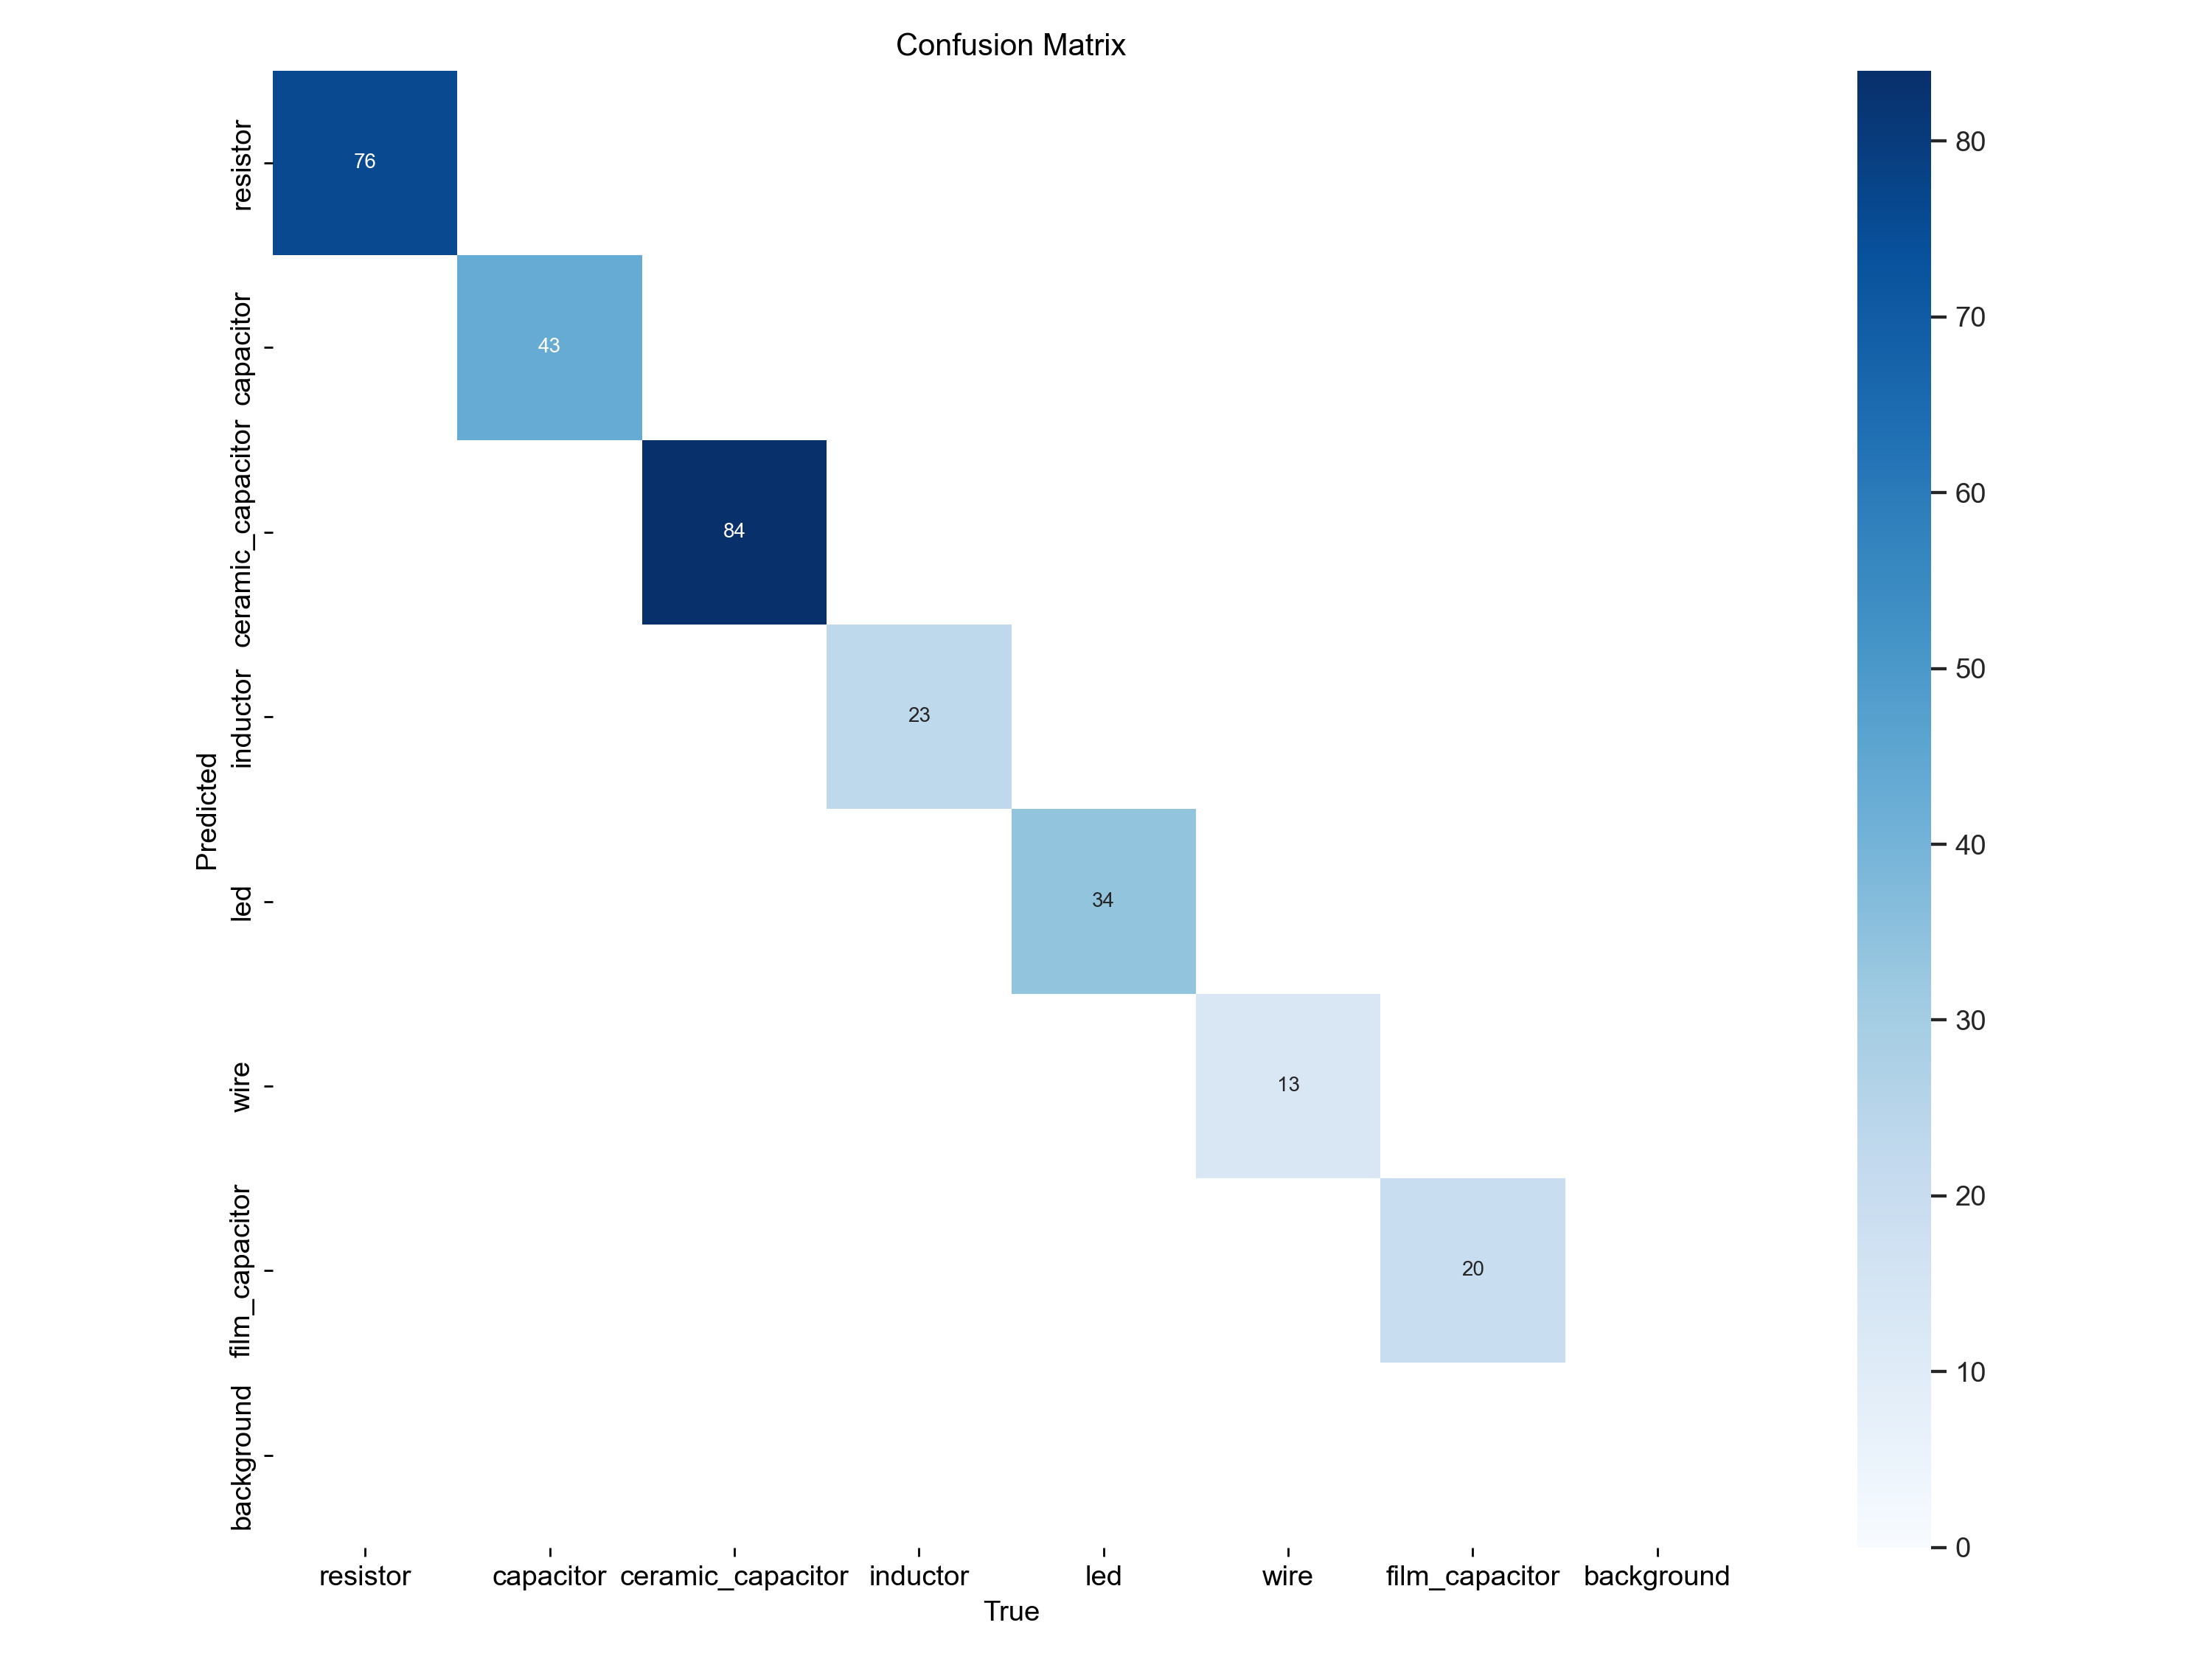
\includegraphics[width=0.8\textwidth]{imgs/graphs/confusion_matrix_final_valtest.png}
  \caption{Unnormalised confusion matrix for the validation and test set}
  \label{fig:final-model-confusion-matrix}
\end{figure}

This again is an exceptional result with no false positives or false negatives, and an mAP\raisebox{-1pt}{\textsuperscript{50-95}} of 82.8\%. The model is able to detect all components in the test set, and is able to classify them correctly. The model is able to generalise well to the test set, and is able to detect components that it has not seen before. In terms of the requirements of the project, the model is able to classify components with a high degree of accuracy.

  
  \todo{talk about tensor board}
  \todo{show metrics}
  
On the GTX 3080 Ti, 
  
Interestingly, if Class Loss is set to 1.0, Box Loss is set to 4.0, and DFL is set to 1.5, the model converges in around ~15 epochs, taking only ~2 minutes to train. However, the model's performance is slightly impacted, calculating metrics on the test set yields an mAP\raisebox{-1pt}{\textsuperscript{50-95}} of 77.8\%, but it was decided that the time savings were not worth it given it was only a few minutes of training time.

\todo{show pictures of model in action}

\subsubsection{Resistor Value Detection Model}
As discussed in \autoref{sec:resistor-value-detection}, the resistor value detection model is a standard YOLOn model trained on images produced by running inference on all resistor images with the component detection model and then cropping the bounding boxes. This meant that there were only 259 images in the dataset, which was then split 80-20 for training and validation; a test set was not used as the dataset was too small. This left only 207 images for training, and 52 images for validation.

\begin{figure}[H]
  \centering
  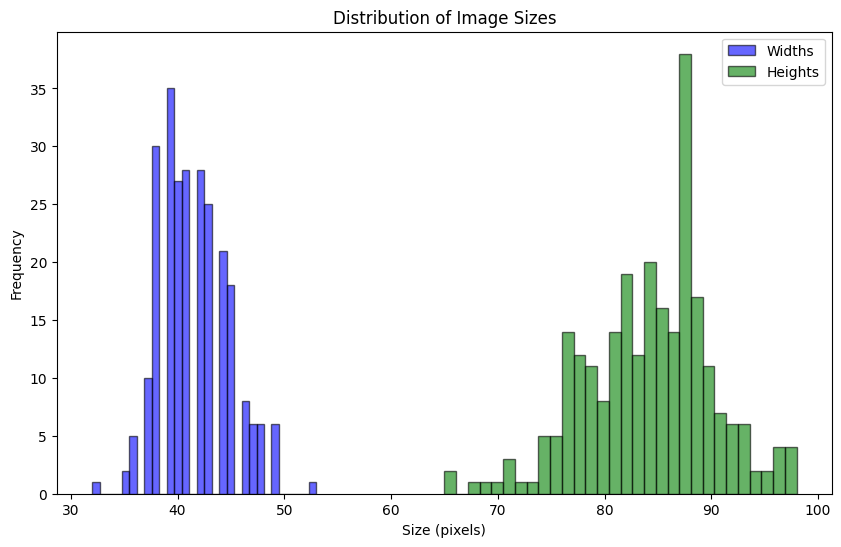
\includegraphics[width=0.8\textwidth]{imgs/graphs/pixel_distrib.png}
  \caption{Distribution of image widths and heights}
  \label{fig:pixel-distrib}
\end{figure}

As the images are generated from the component detection model, the image size is no longer fixed, but instead varies based on the size of the bounding box. The distribution of image sizes is shown in \autoref{fig:pixel-distrib}, where the image sizes vary from 32x65 to 53x98. Due to this, a training parameter was set that would resize all images to a larger size of 128x128, to ensure that the model always works with the same size images.

However, due to the small image sizes and the small dataset, the model only achieved

\subsubsection{Inference Latency}
The inference latency of the model is crucial to the system's performance, as the system must be able to classify components in real-time. The Ultralytics and DeepSparse Python libraries come with their own benchmarking capabilities, and they were used to measure the model's performance. The benchmarks were performed on the Raspberry Pi 4, as this is the intended deployment platform for the system. The benchmarks were performed on the YOLO-OBB model, as it more complex than the standard YOLO model used for the resistor value classification model, and thus should be on the lower end of the performance spectrum.

 % Code block
\begin{minipage}[H]{\textwidth}
  \centering
  \begin{minted}[linenos, fontsize=\footnotesize, breaklines, bgcolor=bg]{bash}
YOLOv8n-obb summary (fused): 187 layers, 3079364 parameters, 0 gradients, 8.3 GFLOPs
val: Scanning /home/dietpi/MEngFYP/datasets/full/current/labels/test.cache... 98 images, 7 backgrounds, 0 corrupt: 100%|----------| 105/105 [00:00<?, ?i
                 Class     Images  Instances      Box(P          R      mAP50  mAP50-95): 100%|%|----------| 105/105 [03:10<00:00,  1.81s/it]
                   all        105         98      0.971          1      0.995      0.793
       {0: 'resistor'}         25         25      0.989          1      0.995      0.819
      {1: 'capacitor'}         17         17      0.983          1      0.995       0.85
    {2: 'ceramic_cap'}         27         27      0.957          1      0.995      0.784
      {3: 'inductors'}          7          7      0.975          1      0.995      0.882
           {7: 'leds'}         13         13      0.981          1      0.995      0.882
           {8: 'wire'}          2          2      0.966          1      0.995      0.499
      {10: 'film_cap'}          7          7      0.949          1      0.995      0.837
Speed: 5.5ms preprocess, 1762.0ms inference, 0.0ms loss, 5.3ms postprocess per image
Results saved to runs/obb/val6
  \end{minted}
  \captionof{listing}{YOLO model inference latency on Raspberry Pi 4}
  \label{code:inference-latency}
\end{minipage}

As shown in \autoref{code:inference-latency}, the standard YOLO model takes 1762ms to performance inference; this translates to ~0.53FPS on the Pi, which is not suitable for real-time object detection. 

% Code block
\begin{minipage}[H]{\textwidth}
  \centering
  \begin{minted}[linenos, fontsize=\footnotesize, breaklines, bgcolor=bg]{bash}
'engine': "ORTEngine
onnx_file_path: ./src/vision/models/final/classifier.onnx  batch_size: 1...
'benchmark_result': {'scenario': 'singlestream', 'items_per_sec': 0.9651499692166781, 'seconds_ran': 60.094287778999956, 'iterations': 58, 'median': 727.9371934999972, 'mean': 1036.078450206897, 'std': 592.0563771426215, '25.0%': 552.4718009999958, '50.0%': 727.9371934999972, '75.0%': 1564.6943927500274, '90.0%': 2038.2221947999483, '95.0%': 2091.3465085999687, '99.0%': 2292.9438349999714, '99.9%': 2342.975698999978}, 'fraction_of_supported_ops': None
  \end{minted}
  \captionof{listing}{Onnxruntime model inference latency on Raspberry Pi 4}
  \label{code:onnx-inference-latency}
\end{minipage}

\autoref{code:onnx-inference-latency} shows the inference latency of the model using the Onnxruntime library \cite{onnxruntime}, which is a popular library for running ONNX models. ONNX (Open Neural Network Exchange) is an open-source format for AI models, and is supported by a wide range of libraries and frameworks. The model takes 1036ms to perform inference, which translates to ~0.96FPS on the Pi, an improvement of 81.1\% over the standard YOLO model. This is a significant improvement, however it is still not suitable for real-time object detection.

% Code block
\begin{minipage}[H]{\textwidth}
  \centering
  \begin{minted}[linenos, fontsize=\footnotesize, breaklines, bgcolor=bg]{bash}
    'engine': 'deepsparse.engine.Engine:
    onnx_file_path: ./src/vision/models/final/classifier.onnx batch_size: 1...
    'benchmark_result': {'scenario': 'singlestream', 'items_per_sec': 1.6153408297780283, 'seconds_ran': 60.04924670499986, 'iterations': 97, 'median': 414.9715189998915, 'mean': 619.0319354845434, 'std': 360.0698332691641, '25.0%': 404.8420740000438, '50.0%': 414.9715189998915, '75.0%': 714.750333000211, '90.0%': 1199.7598698000731, '95.0%': 1420.3843886001316, '99.0%': 1713.9762652400166, '99.9%': 1744.4832248240787}, 'fraction_of_supported_ops': 0.9926
  \end{minted}
  \captionof{listing}{Inference latency of the model using the DeepSparse library}
  \label{code:deepsparse-inference-latency}
\end{minipage}

The DeepSparse library \cite{deepsparse} takes an ONNX model and uses its own engine to perform infernece at higher speeds. Using the library, the model is able to perform inference at 619ms, which translates to ~1.62FPS on the Pi, an improvement of 55.2\% over the standard Onnxruntime model, and an improvement of 203.8\% over the standard YOLO model. This is a significant improvement, and the model is now able to perform inference at a speed that is suitable for real-time object detection.

With these results, the Computer Vision system has met the requirements of the project, and is able to classify components in real-time. The system is able to detect components with a high degree of accuracy, and is able to classify them correctly.